\section{Examples}
In this section we present a set of minimal examples 
that demonstrate how to use Pigeons.jl for sampling. 
We also direct readers to our growing list of examples at InferHub 
(\url{https://julia-tempering.github.io/InferHub/}), which hosts a growing collection of posterior 
distributions with an emphasis on difficult (non-log-concave) problems.

\medskip
We begin by installing the latest official release of Pigeons.jl: 
\begin{lstlisting}[language = Julia]
using Pkg; Pkg.add("Pigeons")
\end{lstlisting}


\subsection{Targets}
To use Pigeons.jl, we must specify a target distribution, given by $\gamma$ 
in \cref{eq:normalizing_constant}.
Numerous possible types of target distributions are supported, including 
custom probability densities (specified up to a normalizing constant) written in Julia.
We also allow to interface with models written in common probabilistic programming 
languages, including:
\begin{itemize}
    \item Turing.jl \cite{ge2018turing} models (\texttt{TuringLogPotential})
    \item Stan \cite{carpenter2017stan} models (\texttt{StanLogPotential})
    \item Comrade.jl\footnote{\url{https://github.com/ptiede/Comrade.jl}} 
      models for black hole imaging (\texttt{ComradeLogPotential})
    \item Non-Julian models with foreign-language Markov chain Monte Carlo (MCMC) code 
    (e.g. Blang \cite{bouchard2022blang} code for phylogenetic inference over combinatorial spaces) 
\end{itemize}
Additional targets are currently being accommodated and will be 
introduced to Pigeons.jl in the near future.

\medskip 
In what follows, we demonstrate how to use Pigeons with a Julia Turing model 
applied to a non-identifiable ``coinflip'' data set, modified from the example
at \url{https://turing.ml/v0.22/docs/using-turing/quick-start}. 
The Bayesian model can be formulated as 
\[
  \label{eq:coinflip}
  p_1, p_2 &\stackrel{iid}{\sim} U(0, 1) \\    
  Y \mid p_1, p_2 &\sim \text{Binomial}(n, p_1 p_2).
\]
The random variable $Y$ is the number of heads observed on $n$ coin flips
where the probability of heads is $p_1 p_2$.  
This model is non-identifiable, meaning that it is not possible to distinguish 
the effects of the two different parameters $p_1$ and $p_2$. As a consequence, 
the target distribution exhibits a complicated structure, as displayed in 
\cref{fig:coinflip_posterior}.
The density of interest corresponding to this model is 
\[
  \pi(p_1, p_2) &= \gamma(p_1, p_2)/Z,
\] 
where 
\[ 
  \gamma(p_1, p_2) &= 
    \binom{n}{y} (p_1 p_2)^y (1-p_1 p_2)^{n-y} I[p_1, p_2 \in [0,1]] 
    \label{eq:coinflip_density} \\
  Z &= \int_0^1 \int_0^1 \gamma(p_1, p_2) \, \dee p_1 \, \dee p_2. \label{eq:coinflip_normalization}
\]
The distribution $\pi$ is also known as the \emph{posterior distribution} in 
Bayesian statistics.

\begin{figure}[t]
    \centering 
    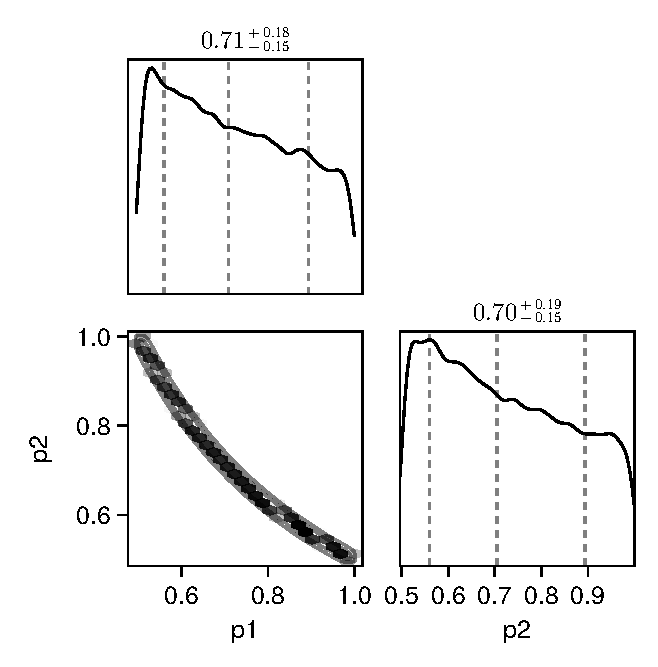
\includegraphics[width=0.5\textwidth]{../img/coinflip_posterior.pdf}
    \caption{Posterior distribution for the model given by \cref{eq:coinflip} 
    with $n=100,000$ coin flips and $y=50,000$ observed heads, 
    estimated using $2^{17}$ samples from Pigeons.jl. 
    We present the pairwise plot for $p_1$ and $p_2$, as well as the estimated 
    densities of the marginal of the posterior for each of the two parameters.
    Note that because the model is non-identifiable, as we collect more data the 
    posterior distribution concentrates around the curve $p_1 p_2 = 0.5$, instead 
    of a single point, assuming that the true probability of observing heads 
    is 0.5.}
    \label{fig:coinflip_posterior}
\end{figure}

\medskip 
Suppose that we perform $n=100,000$ coin tosses and observe 
$y=50,000$ heads.
We would like to obtain samples from our posterior, $\pi$, having collected this data.
We begin by installing Turing
\begin{lstlisting}[language = Julia]
Pkg.add("Turing")
\end{lstlisting}
and then defining our Turing model and storing it in the variable \texttt{model}:
\begin{lstlisting}[language = Julia]
using Turing
@model function coinflip(n, y)
    p1 ~ Uniform(0.0, 1.0)
    p2 ~ Uniform(0.0, 1.0)
    y ~ Binomial(n, p1 * p2)
    return y
end
model = coinflip(100000, 50000)
\end{lstlisting}

From here, it is straightforward to sample from the density given by 
\cref{eq:coinflip_density} up to a normalizing constant.
We use non-reversible parallel tempering 
\cite{syed2021nrpt,syed2021paths,surjanovic2022vpt,surjanovic2024ergodicity} (PT), Pigeons.jl's 
state-of-the-art sampling algorithm, to sample from the target distribution.
PT comes with several tuning parameters and \cite{syed2021nrpt} describe how 
to select these parameters effectively, which Pigeons.jl implements under the hood.
We also specify that we would like to store 
the obtained samples in memory to be able to produce trace-plots, as well 
as some basic online summary statistics of the target distribution and useful 
diagnostic output by specifying 
\texttt{record = [traces, online, round\_trip, Pigeons.timing\_extrema, Pigeons.allocation\_extrema]}.
It is also possible to leave the \texttt{record} argument empty and reasonable defaults 
will be selected for the user.
The code below runs Pigeons.jl on one machine with one thread.
We use the default values for most settings, however 
we explain later how one can obtain improved performance by setting 
arguments more carefully (see \cref{sec:additional_options}).
\begin{lstlisting}[language = Julia]
using Pigeons
pt = pigeons(
    target = TuringLogPotential(model), 
    record = [
        traces, online, round_trip, 
        Pigeons.timing_extrema, 
        Pigeons.allocation_extrema])
\end{lstlisting}
Note that to convert the Turing model into an appropriate Pigeons.jl target for sampling, 
we pass the model as an argument to \texttt{TuringLogPotential()}.
Once we have stored the PT output in the variable \texttt{pt} we can 
access the results, as described in the following section. 
The standard output after running the above code chunk is displayed in \cref{fig:standard_out}
and explained in the next section. 
For purposes of comparison, we also run a traditional 
(single-chain Markov chain Monte Carlo) method. 

\begin{figure*}[t]
    \centering
    \begin{lstlisting}
          --------------------------------------------------------------------------------------
            #scans    restarts      Λ        time(s)    allc(B)  log(Z₁/Z₀)   min(α)     mean(α)
          ---------- ---------- ---------- ---------- ---------- ---------- ---------- --------- 
                  2          0       1.04      0.383   3.48e+07  -4.24e+03          0      0.885
                  4          0       4.06    0.00287   1.79e+06      -16.3   4.63e-06      0.549
                  8          0       3.49    0.00622   3.55e+06      -12.1      0.215      0.612
                 16          0       2.68     0.0161   7.46e+06      -10.2      0.518      0.703
                 32          0       4.29     0.0353   1.37e+07      -11.8      0.222      0.524
                 64          3       3.17     0.0699   2.86e+07      -11.5      0.529      0.648
                128          8       3.56      0.139   5.53e+07      -11.5      0.523      0.605
                256         12       3.38      0.241    1.1e+08      -11.6      0.526      0.625
                512         37       3.48      0.473   2.22e+08        -12      0.527      0.614
           1.02e+03         77       3.55      0.895   4.46e+08      -11.8      0.571      0.605
          --------------------------------------------------------------------------------------
    \end{lstlisting}
    \caption{Standard output provided by Pigeons.jl. 
    Rows indicate tuning rounds of the PT algorithm with an exponentially increasing number 
    of PT iterations (\texttt{\#scans}). Columns indicate various useful diagnostics, 
    such as the number of allocations per round, time (in seconds), and estimates 
    of the log of the normalization constants. 
    The output is described in greater detail in \cref{sec:PT_diagnostics}
    and has been modified to exclude columns that are not described in the paper.}
    \label{fig:standard_out}
\end{figure*}


\subsubsection{Other targets}
As mentioned previously, it is also possible to specify targets with custom 
probability densities, as well as Stan and Turing models. 
Additionally, suppose we have some code implementing vanilla MCMC, written 
in an arbitrary ``foreign'' language such as C++, Python, R, Java, etc. 
Surprisingly, it is very simple to bridge such code with Pigeons.jl. 
The only requirement on the foreign language is that it supports 
reading the standard input and writing to the standard output, 
as described in our online documentation.


\subsection{Outputs}
Pigeons.jl provides many useful types of output, such as: plots of samples from 
the distribution, estimates of normalization constants, summary statistics of 
the target distribution, and various other diagnostics. 
We describe several examples of possible output below.


\subsubsection{Standard output}
An example of the standard output provided by Pigeons.jl is displayed in \cref{fig:standard_out}. 
Each row of the table in the output indicates a new tuning round in parallel tempering, 
with the \texttt{\#scans} column indicating the number of scans/samples in 
that tuning round. 
During these tuning rounds, Pigeons.jl searches for optimal values of certain PT 
tuning parameters. Other outputs include: 
\begin{itemize}
    \item \texttt{restarts}: a higher number is better. 
    Informally, PT performs well at sampling from high-dimensional and/or multi-modal 
    distributions by pushing samples from an easy-to-sample distribution (the reference) 
    to the more difficult target distribution. 
    A tempered restart happens when a sample from the reference successfully 
    percolates to the target. (See the subsequent sections for a more detailed description 
    of parallel tempering.) 
    When the reference supports i.i.d.~sampling, tempered restarts 
    can enable large jumps in the state space. 

    \item \texttt{$\Lambda$}: the global communication barrier, as described in \cite{syed2021nrpt}, 
    which measures the inherent difficulty of the sampling problem.
    A rule of thumb to configure the number of PT chains is also 
    given by \cite{syed2021nrpt}, where they suggest that stable performance 
    should be achieved when the number of chains is set to roughly 2$\Lambda$.
    See \cref{sec:PT_diagnostics} for more information.

    \item \texttt{time} and \texttt{allc}: the time (in seconds) and number of 
    allocations (in bytes) used in each round.

    \item \texttt{$\log(Z_1/Z_0)$}: an estimate of the 
    logarithm of the ratio of normalization constants between the target and the reference. 
    In many cases, $Z_0 = 1$.

    \item \texttt{min($\alpha$)} and \texttt{mean($\alpha$)}: minimum and average swap 
    acceptance rates during the communication phase across the PT chains.
    See \cref{sec:PT} for a description of PT communication.
\end{itemize}


\subsubsection{Plots}
It is straightforward to obtain plots of samples from the target distribution, 
such as trace-plots, pairwise plots, and density plots of the marginals. 

\medskip 
To obtain posterior densities and trace-plots, we first 
make sure that we have the third-party 
MCMCChains.jl\footnote{\url{https://github.com/TuringLang/MCMCChains.jl}}, 
StatsPlots.jl\footnote{\url{https://github.com/JuliaPlots/StatsPlots.jl}}, and 
PlotlyJS.jl\footnote{\url{https://github.com/JuliaPlots/PlotlyJS.jl}} 
packages installed via
\begin{lstlisting}[language=Julia]
Pkg.add("MCMCChains", "StatsPlots", "PlotlyJS")
\end{lstlisting}

With the \texttt{pt} output object from before for our non-identifiable coinflip model, 
we can run the following:
\begin{lstlisting}[language=Julia]
using MCMCChains, StatsPlots, PlotlyJS
plotlyjs()
samples = Chains(
    sample_array(pt), variable_names(pt))
my_plot = StatsPlots.plot(samples)
display(my_plot)
\end{lstlisting}
The output of the above code chunk is an interactive plot that can be zoomed in or out
and exported as an HTML webpage. 
A modified static version of the output for the first parameter, $p_1$, 
is displayed in the top panel of \cref{fig:trace_density_plots},
along with a comparison to the output from a single-chain algorithm in the bottom 
panel of the same figure.

\begin{figure*}[t]
    \centering
    \begin{minipage}{0.45\textwidth}
      \centering
      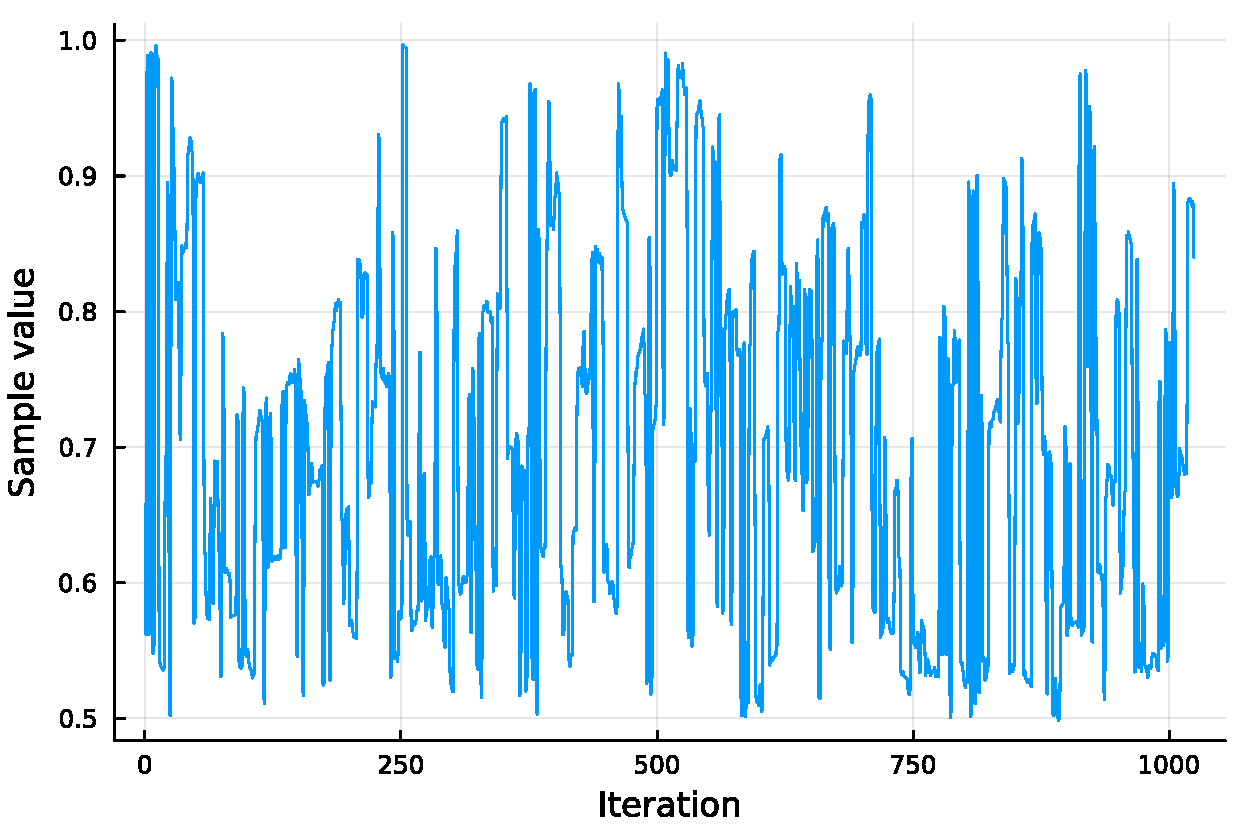
\includegraphics[width=\textwidth]{../img/trace_density_plots_pt.pdf}
    \end{minipage}
    \begin{minipage}{0.45\textwidth}
      \centering
      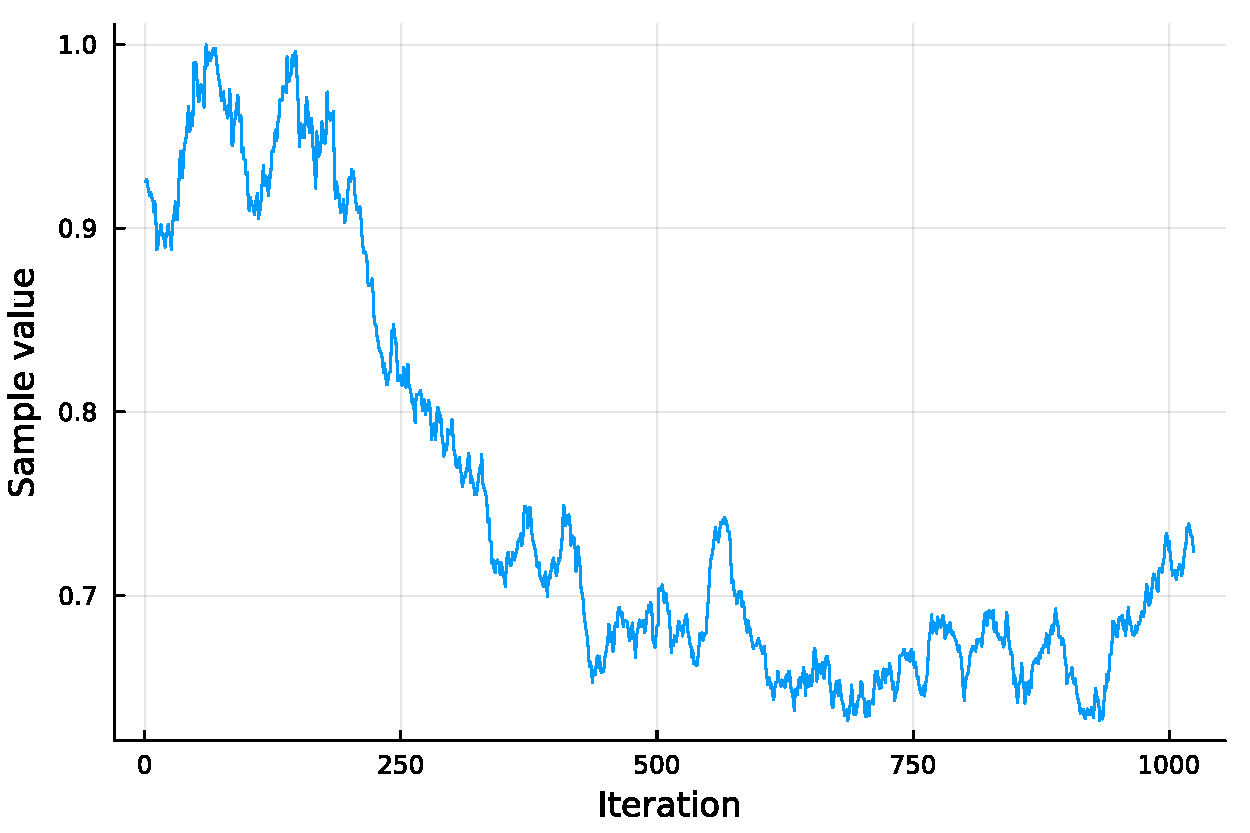
\includegraphics[width=\textwidth]{../img/trace_density_plots_single_chain.pdf}
    \end{minipage}
    \caption{
        Trace-plots for the first parameter, $p_1$, in the 
        non-identifiable coinflip Turing model.
        \textbf{Left:} Samples from Pigeons.jl using PT with 10 chains. Note that the 
        trace-plot indicates fast mixing/exploration across the state space.
        \textbf{Right:} Single-chain Markov chain Monte Carlo. Note that the 
        trace-plot explores the state space much more slowly when we do not use PT.
    }
    \label{fig:trace_density_plots}
\end{figure*}

\medskip 
To obtain pair plots, we add the 
PairPlots.jl\footnote{\url{https://github.com/sefffal/PairPlots.jl}}
and CairoMakie.jl\footnote{\url{https://github.com/JuliaPlots/CairoMakie.jl}}
packages:
\begin{lstlisting}[language=Julia]
Pkg.add("PairPlots", "CairoMakie")
\end{lstlisting}
and then run
\begin{lstlisting}[language=Julia]
using PairPlots, CairoMakie
my_plot = PairPlots.pairplot(samples) 
display(my_plot)
\end{lstlisting}
The output of the above code chunk with an increased number of samples 
is displayed in \cref{fig:coinflip_posterior}.
\footnote{The code chunk above only works with Julia 1.9.}


\subsubsection{Estimate of normalization constant}
The (typically unknown) constant $Z$ in \cref{eq:normalizing_constant} is 
referred to as the \emph{normalization constant}. 
In many applications, it is useful to approximate this constant. 
For example, in Bayesian statistics, this corresponds to the 
marginal likelihood and can be used for model selection. 

\medskip 
As a side-product of PT, we automatically obtain an approximation to the natural 
logarithm of the normalization constant. This is done automatically using the 
stepping stone estimator \cite{xie2011improving}.
The estimate can be accessed using
\begin{lstlisting}[language=Julia]
stepping_stone(pt)
\end{lstlisting}
In the case of the normalization constant given by \cref{eq:coinflip_normalization} 
for $n=100,000$ and $y=50,000$, we can exactly obtain its value as $\log(Z) \approx -11.8794$.
Note that this is very close to the output provided in \cref{fig:standard_out}.


\subsubsection{Online statistics}
\label{sec:online_stats}
Pigeons has facilities to support cases requiring large memory. For instance, we
allow for the computation of online statistics, as well as off-memory sample storage.
Having specified the use of the \texttt{online} recorder in our call to \texttt{pigeons()}, 
we can output some basic summary statistics of the marginals of our target distribution. 
For instance, it is straightforward to estimate the mean and variance of each 
of the marginals of the target with 
\begin{lstlisting}[language=Julia]
using Statistics
mean(pt); var(pt)
\end{lstlisting}
Other constant-memory statistic accumulators are made available in the 
OnlineStats.jl \cite{day2020onlinestats} package. 
To add additional constant-memory statistic accumulators, we 
can register them via \texttt{Pigeons.register\_online\_type()}, as described in our 
online documentation. For instance, we can also compute constant-memory estimates 
of extrema of our distribution.


\subsubsection{Off-memory processing}
When either the dimensionality of the model or the number of samples is large,
the obtained samples may not fit in memory. 
In some cases it may be necessary to store samples to disk if our statistics of 
interest cannot be calculated online and with constant-memory
(see \cref{sec:online_stats}).
We show here how to save samples to disk when Pigeons.jl is run on a single 
machine. A similar interface can be used over MPI. 

\medskip 
First, we make sure that we set \texttt{checkpoint = true}, which saves a 
snapshot at the end of each round in the directory \texttt{results/all/<unique directory>}
and is symlinked to \texttt{results/latest}.
Second, we make sure that we use the \texttt{disk} recorder 
by setting \texttt{record = [disk]}, along with possibly any other desired recorders.
Accessing the samples from disk can then be achieved in a simple way using the Pigeons.jl 
function \texttt{process\_sample()}.


\subsubsection{PT diagnostics}
\label{sec:PT_diagnostics}
We describe how to produce some key parallel tempering diagnostics from 
\cite{syed2021nrpt}.

\medskip 
The global communication barrier, denoted $\Lambda$ in Pigeons.jl output, can be 
used to approximately inform the appropriate number of chains. 
Based on \cite{syed2021nrpt}, stable PT performance should be achieved when  
the number of chains is set to roughly $2\Lambda$. This can be achieved by 
modifying the \texttt{n\_chains} argument in the call to \texttt{pigeons()}. 
The global communication barrier is shown at each round and can also be accessed 
with 
\begin{lstlisting}[language=Julia]
Pigeons.global_barrier(pt)
\end{lstlisting}

The number of restarts per round can be accessed with 
\begin{lstlisting}[language=Julia]
n_tempered_restarts(pt)
\end{lstlisting}
These quantities are also displayed in \cref{fig:standard_out}. 
Many other useful PT diagnostic statistics and plots can be obtained, as described 
in our full documentation. 


\subsection{Parallel and distributed PT}
One of the main benefits of Pigeons.jl is that it allows users to easily parallelize 
and/or distribute their PT sampling efforts. We explain how to run MPI locally on 
one machine and also how to use MPI when a cluster is available.

\subsubsection{Running MPI locally}
To run MPI locally on one machine using four MPI processes and one thread per process,
use
\begin{lstlisting}[language = Julia]
pigeons(
    target = TuringLogPotential(model), 
    on = ChildProcess(
            n_local_mpi_processes = 4,
            n_threads = 1))
\end{lstlisting}

\subsubsection{Running MPI on a cluster}
Often, MPI is available via a cluster scheduling system. To run MPI over 
several machines:
\begin{enumerate}
    \item In the cluster login node, follow the Pigeons.jl installation instructions
    in our online documentation. 
    \item Start Julia in the login node, and perform a one-time setup by 
    calling \texttt{Pigeons.setup\_mpi()}.
    \item In the Julia REPL running in the login node, run:
\end{enumerate}
\begin{lstlisting}[language = Julia]
pigeons(
    target = TuringLogPotential(model), 
    n_chains = 1_000,
    on = MPI(n_mpi_processes = 1_000, 
             n_threads = 1))
\end{lstlisting}
The code above will start a distributed PT algorithm with 1,000 chains on 1,000 
MPI processes each using one thread.
Note that for the above code chunks involving \texttt{ChildProcess()} and 
\texttt{MPI()} to work, it may be necessary to specify dependencies in their 
function calls.


\subsection{Additional options}
\label{sec:additional_options}
In the preceding example we only specified the target distribution and let 
Pigeons.jl decide on default values for most other settings of the inference engine. 
There are various settings we can change, including: 
the random seed (\texttt{seed}), the number of PT chains (\texttt{n\_chains}), 
the number of PT tuning rounds/samples (\texttt{n\_rounds}), 
and a variational reference distribution family (\texttt{variational}), among other settings.
For instance, we can run 
\begin{lstlisting}[language = Julia]
pigeons(
    target = TuringLogPotential(model),
    n_rounds = 10, 
    n_chains = 10,
    variational = GaussianReference(),
    seed = 2
)
\end{lstlisting}
which runs PT with the same Turing model target as before and explicitly states 
that we should use 10 PT tuning rounds with 10 chains (described below). 
In the above code chunk we also specify that we would like to use a 
Gaussian variational reference distribution.
That is, the reference distribution is chosen from a multivariate Gaussian family 
that lies as close as possible to the target distribution in order to improve 
the efficiency of PT. We refer readers to \cite{surjanovic2022vpt} for more details.
When only continuous parameters are of interest, we encourage users to consider 
using \texttt{variational = GaussianReference()} and setting \texttt{n\_chains\_variational = 10}, 
for example, as the number of restarts may substantially increase with these settings.

